\begin{frame} %-----------------------------------
\frametitle{Experiments: Images}


    MNIST digits sum: \textit{"Sample two MNIST images whose digit labels sum up to 10"}

    $$\bigvee_{i=1}^{9} \text{{class}}(\myvec{x}, i) \land \text{{class}}(\myvec{y}, 10-i) $$

        Where "class" is a pretrained classifier.


    \begin{figure}[htbp!] 
    \centering    
    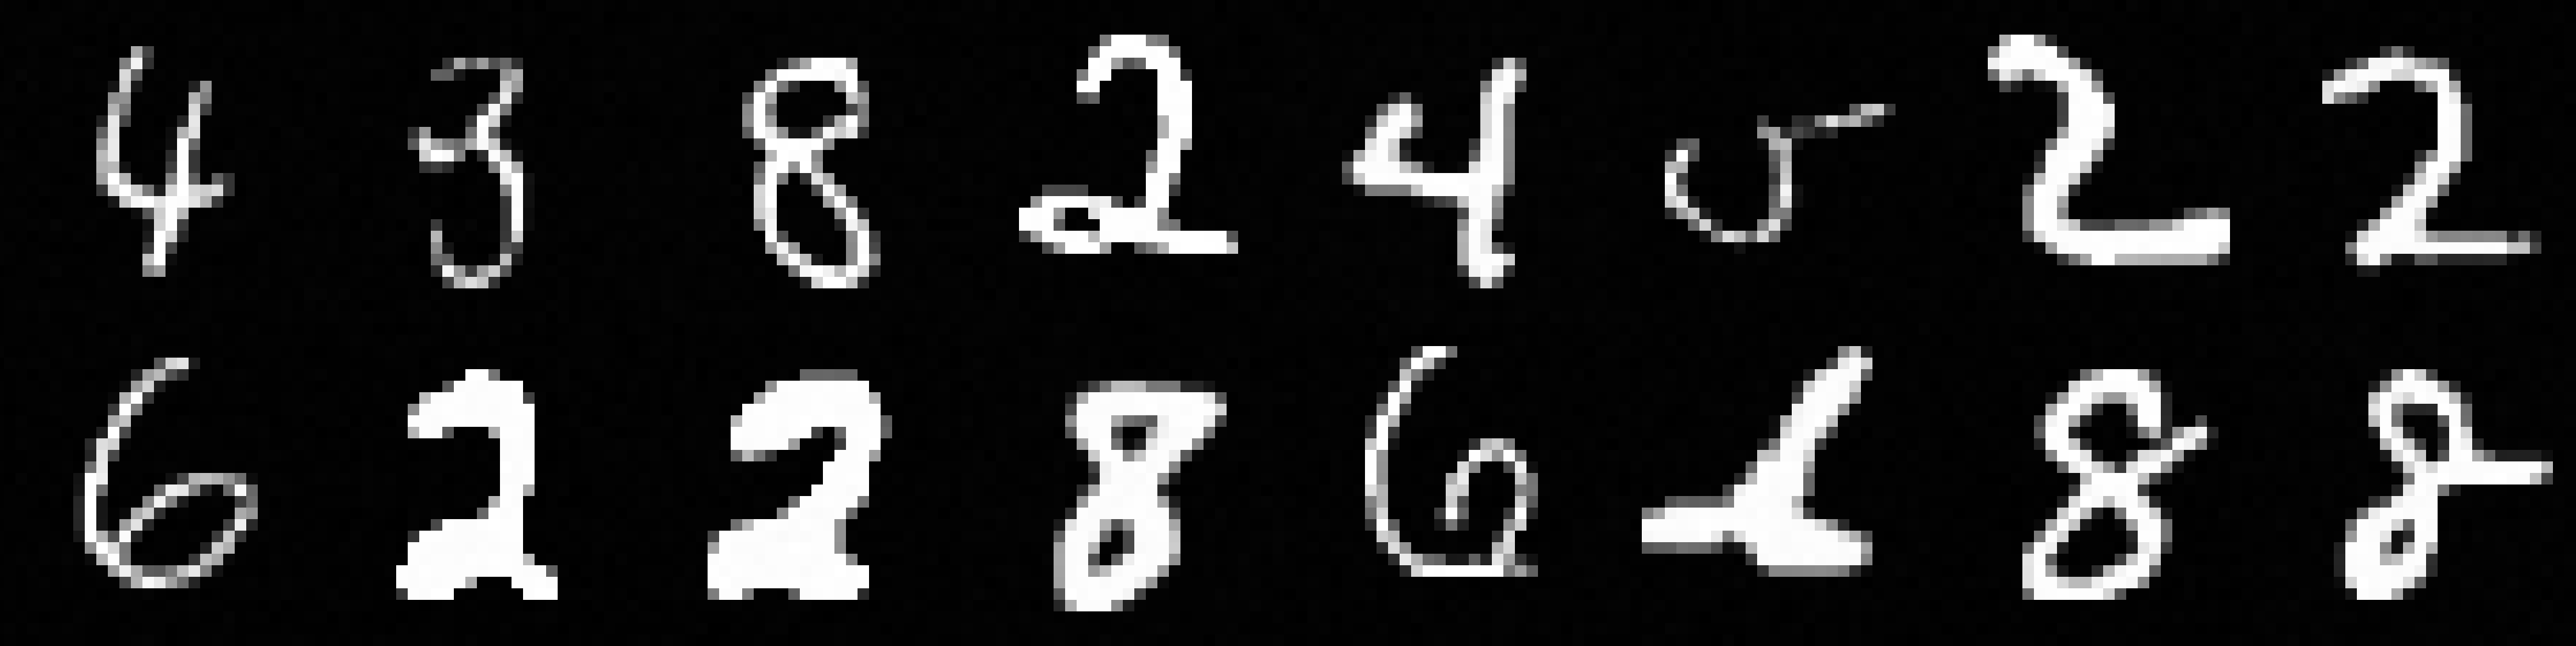
\includegraphics[width=0.8\textwidth]{assets/images/passaggio_anno/mnist_digits_sum.png}
    \end{figure}


    According to the classifier $\approx 96\%$ of pairs sum up to 10, but only 2-8, 6-4 pairs are generated.

\end{frame} %-----------------------------------

\begin{frame} %-----------------------------------
\frametitle{Comparison with Universal Guidance}

\begin{itemize}
    \item Universal Guidance (\cite{bansal2023universal}) is probably the state of the art for plug-and-play conditioning.

    \item Originally applied to imaging problems
    
    \item Synthesis of previous optimization-based approaches for solving inverse problems with diffusion models

    \item Oversimplifying, it involves at each time step an optimization of the denoising prediction $\myvec{x}_0$ (that is a linear transformation of the score), in order to make it satisfy the constraint $c(\myvec{x}_0)$.
    \bigskip

    \begin{figure} 
    \centering    
    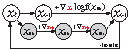
\includegraphics[width=0.5\textwidth]{assets/images/universal_guidance_cartoon.pdf}
    \end{figure}

\end{itemize}

\end{frame} %-----------------------------------


\begin{frame} %-----------------------------------
\frametitle{Comparison with Universal Guidance}

Universal guidance fails in two of the tasks we tested (White wine and eSIRS bridging). However, it performs better on one of the tasks based on images.

    \bigskip

    % \begin{figure} 
    % \centering    
    % 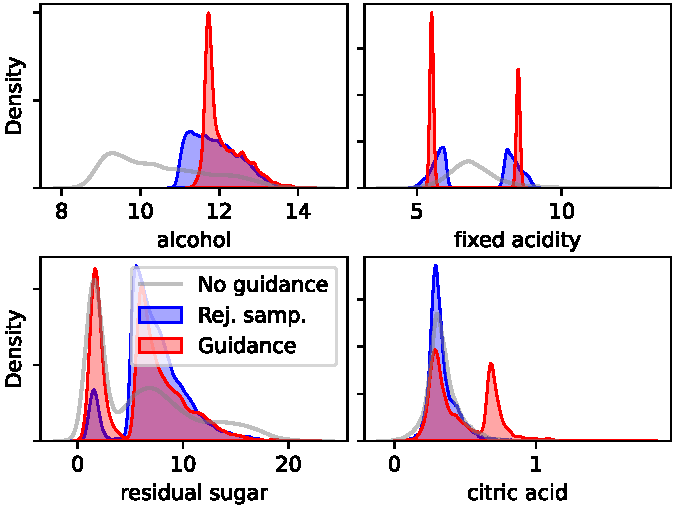
\includegraphics[width=0.5\textwidth]{assets/images/white_wine_fw_bw.pdf}
    % \end{figure}

    \begin{table}[ht]    
    \begin{tabular}{@{}lcccc@{}}
    \toprule
    \multicolumn{1}{c}{\multirow{2}{*}{Method}} & \multicolumn{2}{c}{White wine} & \multicolumn{2}{c}{eSIRS bridging} \\ \cmidrule(l){2-5} 
    \multicolumn{1}{c}{} & \textbf{Avg TV} & \textbf{Max TV} & \textbf{Avg TV} & \textbf{Max TV} \\ \midrule
    \textbf{Ours}        & \textbf{0.1}    & \textbf{0.15}  & \textbf{0.13}  & \textbf{0.25}  \\
    Univ. Guidance                   & 0.29           & 0.85           & 0.47           & 1.0             \\ \bottomrule
    \end{tabular}
    \end{table}

\end{frame} %-----------------------------------

\begin{frame} %-----------------------------------
\frametitle{Comparison with Universal Guidance}

    Universal Guidance performs better on image problems:
    $$\bigvee_{i=1}^{9} \text{{class}}(\myvec{x}, i) \land \text{{class}}(\myvec{y}, 10-i) $$

    \begin{figure}[htbp!] 
    \centering    
    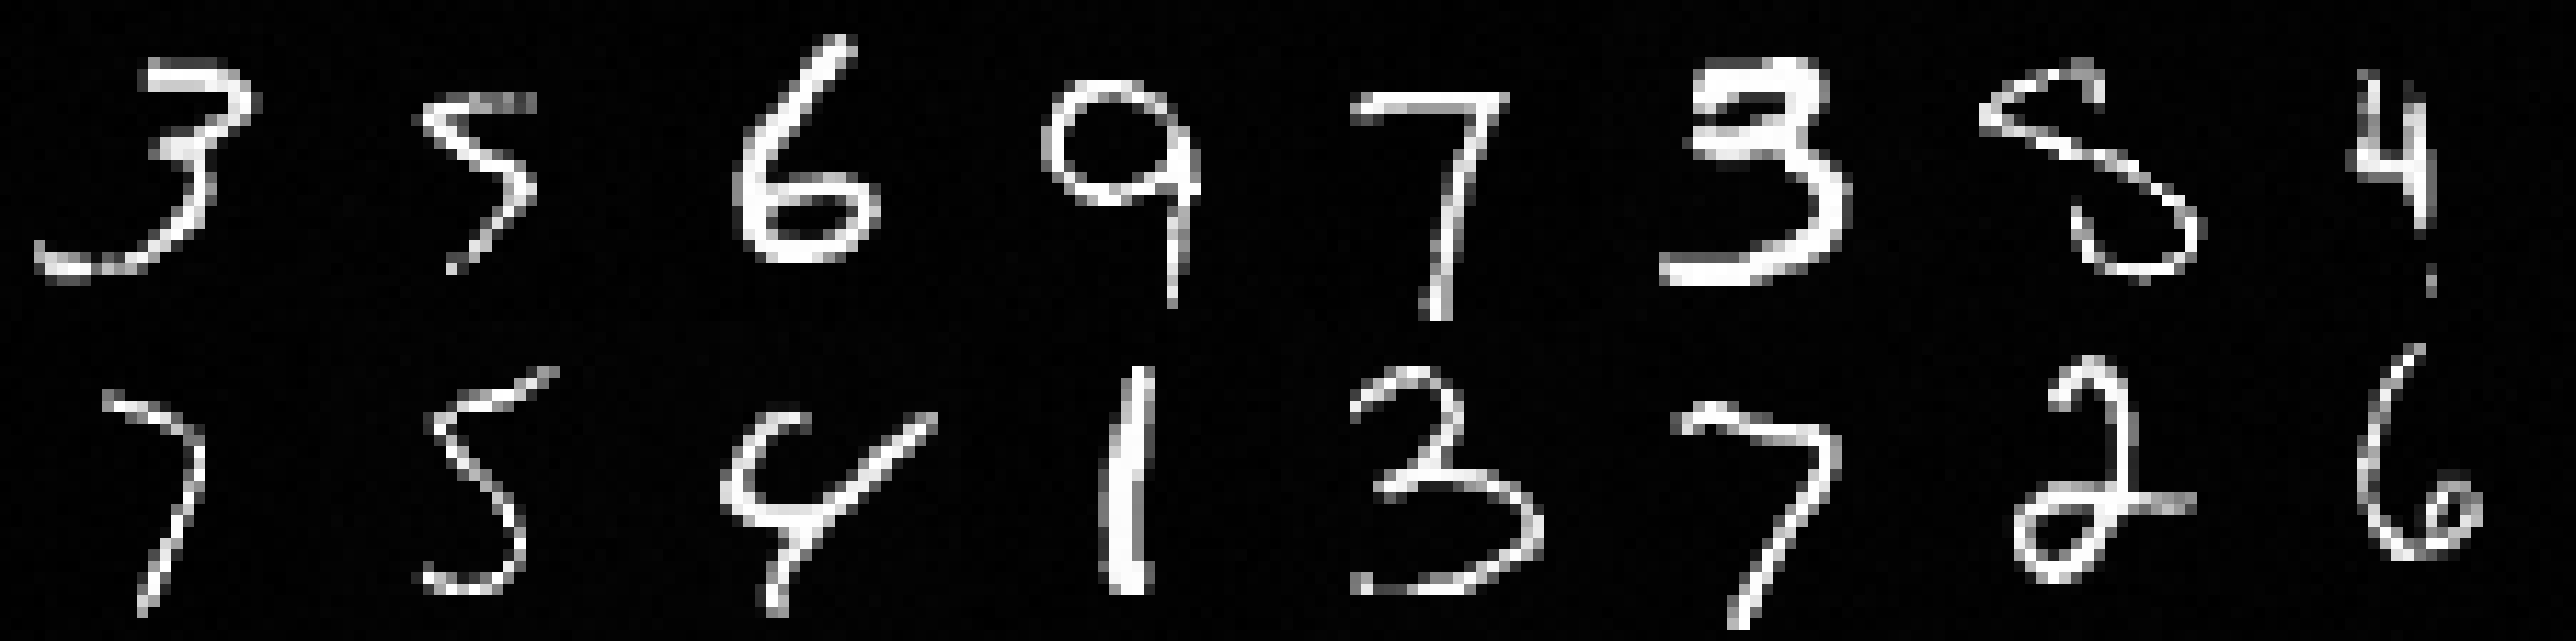
\includegraphics[width=0.8\textwidth]{assets/images/passaggio_anno/mnist_digits_sum_universal_guidance.png}
    \end{figure}

    It is able to generate high quality samples but it misses the correct approximation of the conditional distribution, probably because it involves an optimization phase.  


\end{frame} %-----------------------------------


% -------------------------------------------------------------------------------------
\begin{frame}[fragile]{Datasets Details (1)}

  \scriptsize
  \begin{table}[ht]
\centering
\caption{\small Overview of the datasets used in the experiments, showing for each table of each dataset the number of rows, the number of features (feature columns) and tables referred by foreign keys (the parent tables).}

\begin{tabular}{l l r r l}
\toprule
\textbf{Dataset} & \textbf{Table} & \textbf{\# Rows} & \textbf{\# Features} & \textbf{Foreign Keys} \\
\cmidrule(lr){1-5}
\multirow{2}{*}{AirBnB} 
  & users    & $10,000$  & $15$ & -- \\
  & sessions & $47,217$  & $5$  & users \\
\addlinespace
\cmidrule(lr){1-5}
\multirow{5}{*}{Biodegradability} 
  & molecule & $328$     & $3$  & -- \\
  & group    & $1,736$   & $1$  & -- \\
  & atom     & $6,568$   & $1$  & molecule \\
  & gmember  & $6,647$   & --  & atom, group \\
  & bond     & $6,616$   & $1$  & atom1, atom2 \\
\addlinespace
\cmidrule(lr){1-5}
\multirow{3}{*}{CORA} 
  & paper    & $2,708$   & $1$  & -- \\
  & content  & $49,216$  & $1$  & paper \\
  & cites    & $5,429$   & --  & paper1, paper2 \\
\bottomrule
\end{tabular}


\end{table}

\end{frame}
% -------------------------------------------------------------------------------------


% -------------------------------------------------------------------------------------
\begin{frame}[fragile]{Datasets Details (2)}

  \scriptsize
  \begin{table}[ht]
\centering
\caption{\small Overview of the datasets used in the experiments, showing for each table of each dataset the number of rows, the number of features (feature columns) and tables referred by foreign keys (the parent tables).}

\begin{tabular}{l l r r l}
\toprule
\textbf{Dataset} & \textbf{Table} & \textbf{\# Rows} & \textbf{\# Features} & \textbf{Foreign Keys} \\
\cmidrule(lr){1-5}
\multirow{7}{*}{IMDB MovieLens} 
  & users            & $6,039$    & $3$  & -- \\
  & movies           & $3,832$    & $4$  & -- \\
  & actors           & $98,690$   & $2$  & -- \\
  & directors        & $2,201$    & $2$  & -- \\
  & ratings          & $996,159$  & $1$  & movie, user \\
  & movies2actors    & $138,349$  & $1$  & movie, actor \\
  & movies2directors & $4,141$    & $1$  & movie, director \\
\addlinespace
\cmidrule(lr){1-5}
\multirow{2}{*}{Rossmann} 
  & store      & $1,115$   & $9$  & -- \\
  & historical & $57,970$  & $7$  & store \\
\addlinespace
\cmidrule(lr){1-5}
\multirow{3}{*}{Walmart} 
  & stores    & $45$     & $2$  & -- \\
  & features  & $225$    & $11$ & store \\
  & depts     & $15,047$ & $4$  & store \\
\bottomrule
\end{tabular}


\end{table}

\end{frame}
% -------------------------------------------------------------------------------------


% -------------------------------------------------------------------------------------
\begin{frame}[fragile]{GNN Architecture Details}

\textbf{Core Approach:}
\begin{itemize}
  \item GNNs compute node embeddings $\boldsymbol{\varepsilon}^i$ for each record $i$
  \item Handles heterogeneous graphs with multiple node/edge types
  \item Edge-type-specific convolutions aggregate neighbors by table type
\end{itemize}

\textbf{Two Architecture Variants:}
\begin{columns}[T,onlytextwidth]
  \column{0.48\textwidth}
  \textit{GATv2-based:} \citet{brody2021attentive}
  \begin{itemize}
    \item Attention mechanism
    \item Residual connections
    \item Hidden dim: 100
    \item Used for: AirBnB, Rossmann, Walmart
  \end{itemize}
  
  \column{0.48\textwidth}
  \textit{GIN-based:} \citet{xu2018powerful}
  \begin{itemize}
    \item 3 GIN layers
    \item MLP width: 100
    \item Embedding size: 20 or 50
    \item Used for: CORA, IMDB, Biodegradability
  \end{itemize}
\end{columns}

\end{frame}
% -------------------------------------------------------------------------------------

% -------------------------------------------------------------------------------------
\begin{frame}[fragile]{Table-specific Denoisers}

\textbf{Architecture:}
\begin{itemize}
  \item Each table $k$ has a dedicated MLP denoiser $f^k$ that predicts clean records:
  \begin{equation*}
  \hat{\mathbf{x}}^i_1 = f^{k_i}(\mathbf{x}^i_t, t, \boldsymbol{\varepsilon}^i_t)
  \end{equation*}
  \item \textbf{Inputs}: noisy record $\mathbf{x}^i_t$ + time embedding $t$ + node embedding $\boldsymbol{\varepsilon}^i_t$
  \item \textbf{Design}: Layer Normalization + SiLU activations + linear output
  \item \textbf{Output}: Softmax for categoricals, linear for continuous features
\end{itemize}

\textbf{Hyperparameters:}
\begin{itemize}
  \item 2-3 hidden layers per table
  \item Width: 10-1000 hidden units (dataset-specific)
\end{itemize}

\end{frame}
% -------------------------------------------------------------------------------------

% -------------------------------------------------------------------------------------
\begin{frame}[fragile]{Tuning Node Embedding Size}

\textbf{Key Tradeoff:}
\begin{itemize}
  \item Too large → memorization and privacy leaks
  \item Too small → limited expressiveness
  \item Our choice: 2-10 dimensions (conservative for privacy)
\end{itemize}

\begin{figure}[ht]
    \centering
    \begin{minipage}[b]{0.45\textwidth}
        \centering
        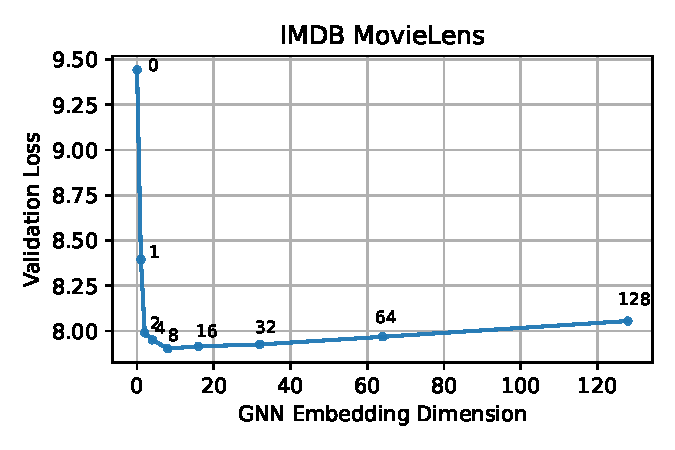
\includegraphics[width=\textwidth]{assets/images/embedding_vs_val_IMDB_MovieLens.pdf}
        
        (a) IMDB MovieLens
    \end{minipage}
    \hfill
    \begin{minipage}[b]{0.45\textwidth}
        \centering
        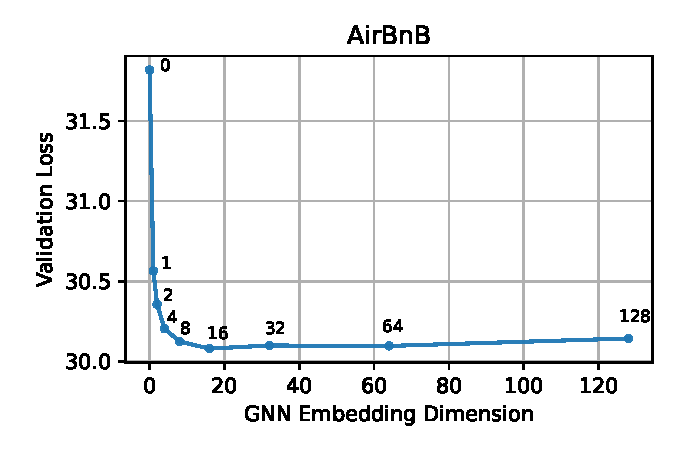
\includegraphics[width=\textwidth]{assets/images/embedding_vs_val_AirBnB.pdf}
        
        (b) Airbnb
    \end{minipage}
    
    \vspace{0.3em}
    Validation loss vs. GNN embedding size (0 = no GNN)
\end{figure}

%\textbf{Observation:} IMDB degrades with larger embeddings; Airbnb less sensitive (different GNN).

\end{frame}
% -------------------------------------------------------------------------------------

\begin{frame}[fragile]{Results: Privacy and Efficiency}
  \begin{itemize}
    \item \textbf{Privacy}: DCR (Distance to Closest Record) analysis does not highlight privacy leaks. Intuitively, we check if generated records are too similar to real records in the training set.
    \item \textbf{Efficiency}: Training and generation are fast. \footnote{on a single NVIDIA RTX A5000}
  \end{itemize}

\begin{table}[h]
\centering
%\caption{Maximum runtime across repetitions for each dataset during experimentation.}
\label{tab:experiment_duration}
\begin{tabular}{l r}
\toprule
\textbf{Dataset Name} & \textbf{Running Time} \\
\midrule
AirBnB                & $10$m $3$s \\
Biodegradability      & $1$m $6$s  \\
CORA                  & $3$m $10$s \\
IMDB MovieLens        & $14$m $25$s \\
Rossmann              & $2$m $57$s \\
Walmart               & $1$m $48$s \\
\bottomrule
\end{tabular}
\end{table}

\end{frame}
% -------------------------------------------------------------------------------------


\begin{frame}[fragile]{wNMIE}

    \begin{columns}
        \column{0.5\textwidth}
            \begin{figure}
                \centering
                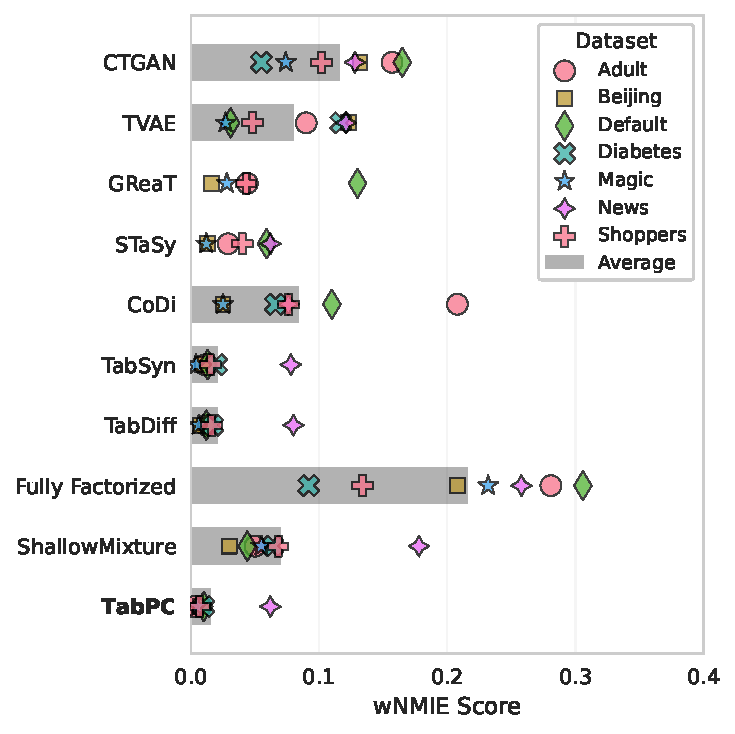
\includegraphics[width=1.00\textwidth]{images/nmi.pdf}
            \end{figure}

        \column{0.5\textwidth}
            
            \begin{itemize}
                \item wNMIWE is not influenced by marginals, fully factorized models perform poorly as expected.
                \item TabPC is competitive with state-of-the-art diffusion-based models.
            \end{itemize}

    \end{columns}

\end{frame}


% -------------------------------------------------------------------------------------

\begin{frame}[fragile]{TabPC: DCR experiment}
  
  \begin{table}[t!]  
    \centering
    \caption{DCR scores (\%). In this table we report the percentage of times the DCR of a synthetic data sample with respect to the training set was lower than the $2\%$ quantile of the empirical distribution of DCRs of the test set. %Values significantly higher than $2\%$ suggest potential privacy leaks. Conversely, values lower than $2\%$ indicate that synthetic samples are farther from training records than test records, which may signal underfitting.
    }
    \label{tbl:dcr002}
    %\small
    \begin{threeparttable}
    {
    \resizebox{\columnwidth}{!}
    {
\begin{tabular}{lrrrrrrr|r}
    \toprule[0.8pt]
     \textbf{Method} & \textbf{Adult} & \textbf{Beijing} & \textbf{Default} & \textbf{Diabetes} & \textbf{Magic} & \textbf{News} & \textbf{Shoppers} & \textbf{Average} \\
    \midrule 
    CTGAN & $0.01${\tiny${\pm 0.000}$} & $0.0${\tiny${\pm 0.000}$} & $0.0${\tiny${\pm 0.000}$} & $0.03${\tiny${\pm 0.01}$} & $0.0${\tiny${\pm 0.000}$} & $0.09${\tiny${\pm 0.02}$} & $0.0${\tiny${\pm 0.000}$} & $0.0186$ \\
    TVAE & $6.41${\tiny${\pm 0.11}$} & $0.0${\tiny${\pm 0.000}$} & $0.06${\tiny${\pm 0.01}$} & $19.55${\tiny${\pm 0.17}$} & $0.01${\tiny${\pm 0.01}$} & $0.22${\tiny${\pm 0.02}$} & $0.02${\tiny${\pm 0.01}$} & $3.7529$ \\
    GReaT & $0.0${\tiny${\pm 0.000}$} & $1.49${\tiny${\pm 0.06}$} & $12.54${\tiny${\pm 0.17}$} & $-$ & $0.35${\tiny${\pm 0.04}$} & $-$ & $10.8${\tiny${\pm 0.35}$} & $-$ \\
    STaSy & $1.1${\tiny${\pm 0.04}$} & $0.44${\tiny${\pm 0.04}$} & $0.56${\tiny${\pm 0.06}$} & $-$ & $0.28${\tiny${\pm 0.04}$} & $0.25${\tiny${\pm 0.03}$} & $0.27${\tiny${\pm 0.05}$} & $-$ \\
    CoDi & $0.06${\tiny${\pm 0.01}$} & $0.0${\tiny${\pm 0.000}$} & $0.0${\tiny${\pm 0.000}$} & $0.0${\tiny${\pm 0.000}$} & $0.03${\tiny${\pm 0.01}$} & $0.0${\tiny${\pm 0.000}$} & $0.0${\tiny${\pm 0.000}$} & $0.0129$ \\
    TabSyn & $1.72${\tiny${\pm 0.07}$} & $0.51${\tiny${\pm 0.05}$} & $1.12${\tiny${\pm 0.05}$} & $0.65${\tiny${\pm 0.02}$} & $0.07${\tiny${\pm 0.02}$} & $0.81${\tiny${\pm 0.05}$} & $1.76${\tiny${\pm 0.12}$} & $0.9486$ \\
    TabDiff & $1.85${\tiny${\pm 0.07}$} & $0.61${\tiny${\pm 0.05}$} & $1.4${\tiny${\pm 0.06}$} & $1.35${\tiny${\pm 0.05}$} & $0.05${\tiny${\pm 0.02}$} & $0.89${\tiny${\pm 0.05}$} & $2.24${\tiny${\pm 0.09}$} & $1.1986$ \\
    \midrule
    Fully Factorized & $0.0${\tiny${\pm 0.000}$} & $0.0${\tiny${\pm 0.000}$} & $0.0${\tiny${\pm 0.000}$} & $0.01${\tiny${\pm 0.000}$} & $0.0${\tiny${\pm 0.000}$} & $0.0${\tiny${\pm 0.000}$} & $0.0${\tiny${\pm 0.000}$} & $0.0014$ \\
    Fully Factorized (P) & $0.04${\tiny${\pm 0.01}$} & $0.08${\tiny${\pm 0.01}$} & $0.0${\tiny${\pm 0.000}$} & $0.01${\tiny${\pm 0.000}$} & $0.0${\tiny${\pm 0.000}$} & $0.0${\tiny${\pm 0.000}$} & $0.0${\tiny${\pm 0.000}$} & $0.0186$ \\
    ShallowMixture & $2.217${\tiny${\pm 0.064}$} & $0.923${\tiny${\pm 0.06}$} & $0.708${\tiny${\pm 0.055}$} & $0.089${\tiny${\pm 0.009}$} & $0.505${\tiny${\pm 0.068}$} & $0.07${\tiny${\pm 0.01}$} & $1.311${\tiny${\pm 0.1}$} & $0.832$ \\
    TabPC & $1.84${\tiny${\pm 0.09}$} & $0.51${\tiny${\pm 0.04}$} & $0.92${\tiny${\pm 0.06}$} & $1.17${\tiny${\pm 0.05}$} & $0.14${\tiny${\pm 0.03}$} & $0.68${\tiny${\pm 0.04}$} & $2.52${\tiny${\pm 0.15}$} & $1.1114$ \\
    \bottomrule[1.0pt]
\end{tabular}
}
    }
    \end{threeparttable}
\end{table}

\end{frame}

% ------------------------------------------------------------

\begin{frame}[fragile]{TabPC: Datasets Details}
  
\begin{table}[ht]
    \centering
    \caption{Dataset statistics. \# Num = number of numerical columns, \# Cat = number of categorical columns, \# Max Cat = max categories in any categorical column. \# Train and \# Test refer to the number of samples in the training and test splits respectively.}
    \label{tbl:exp-dataset}
    \small
    \begin{tabular}{lrrrrrrl}
        \toprule
        \textbf{Dataset} & \textbf{\# Rows} & \textbf{\# Num} & \textbf{\# Cat} & \textbf{\# Max Cat} & \textbf{\# Train} & \textbf{\# Test} & \textbf{Task} \\
        \midrule
        Adult     & $48,842$  & $6$  & $9$  & $42$  & $32,561$ & $16,281$ & Classification \\
        Default   & $30,000$  & $14$ & $11$ & $11$  & $27,000$ & $3,000$  & Classification \\
        Shoppers  & $12,330$  & $10$ & $8$  & $20$  & $11,097$ & $1,233$  & Classification \\
        Magic     & $19,019$  & $10$ & $1$  & $2$   & $17,117$ & $1,902$  & Classification \\
        Beijing   & $43,824$  & $7$  & $5$  & $31$  & $39,441$ & $4,383$  & Regression     \\
        News      & $39,644$  & $46$ & $2$  & $7$   & $35,679$ & $3,965$  & Regression     \\
        Diabetes  & $101,766$ & $9$  & $27$ & $716$ & $81,412$ & $20,354$ & Classification \\
        \bottomrule
    \end{tabular}
\end{table}

\end{frame}
